\documentclass[notes,11pt, aspectratio=169]{beamer}
\usetheme{default}
\usepackage{helvet}
\usepackage[default]{lato}
\usepackage{amsmath}
\usepackage{mathpazo}
\usepackage{hyperref}
\usepackage{lipsum}
\usepackage{multimedia}
\usepackage{graphicx}
\usepackage{tikz}
\usetikzlibrary{arrows.meta, positioning}
\usepackage{multirow}
\usepackage{graphicx}
\usepackage{changepage}
\usepackage{appendixnumberbeamer}
\newcommand{\beginbackup}{
   \newcounter{framenumbervorappendix}
   \setcounter{framenumbervorappendix}{\value{framenumber}}
   \setbeamertemplate{footline}
   {
     \leavevmode%
     \hline
     box{%
       \begin{beamercolorbox}[wd=\paperwidth,ht=2.25ex,dp=1ex,right]{footlinecolor}%
%         \insertframenumber  \hspace*{2ex}
       \end{beamercolorbox}}%
     \vskip0pt%
   }
 }
\newcommand{\backupend}{
   \addtocounter{framenumbervorappendix}{-\value{framenumber}}
   \addtocounter{framenumber}{\value{framenumbervorappendix}}
}
% These are my colors -- there are many like them, but these ones are mine.
\definecolor{blue}{RGB}{0,114,178}
\definecolor{red}{RGB}{213,94,0}
\definecolor{yellow}{RGB}{240,228,66}
\definecolor{green}{RGB}{0,158,115}

\hypersetup{
  colorlinks=false,
  linkbordercolor = {white},
  linkcolor = {blue}
}


%% I use a beige off white for my background
\definecolor{MyBackground}{RGB}{255,253,218}
\setbeamercolor{frametitle}{fg=blue}
\setbeamercolor{title}{fg=black}
\setbeamertemplate{footline}[frame number]
\setbeamertemplate{navigation symbols}{}
\setbeamertemplate{itemize items}{-}
\setbeamercolor{itemize item}{fg=blue}
\setbeamercolor{itemize subitem}{fg=blue}
\setbeamercolor{enumerate item}{fg=blue}
\setbeamercolor{enumerate subitem}{fg=blue}
\setbeamercolor{button}{bg=MyBackground,fg=blue,}
\setbeamercolor{section in toc}{fg=blue}
\setbeamercolor{subsection in toc}{fg=red}
\setbeamersize{text margin left=1em,text margin right=1em}

\newenvironment{wideitemize}{\itemize\addtolength{\itemsep}{0.4em}}{\enditemize}

% Customizing footer to display only the current page number
% Customizing footer: Right-aligned but with some padding from the edge
\setbeamertemplate{footline}{%
  \hfill
  \begin{beamercolorbox}[wd=\paperwidth,ht=0.4cm,dp=0.3cm,right]{footline}%
    \hspace{-1cm} \insertframenumber\hspace{0.2cm} % Adjust the spacing here
  \end{beamercolorbox}%
}

\title{\textcolor{blue}{The economics of infertility:\\ Evidence from reproductive medicine}}

\author{Sarah Bogl \and Jasmin moshfegh \and Petra Persson \and Maria Polyakova}

\institute{\textit{R\&R at QJE}}

\date{April 14, 2025}

\begin{document}

\begin{frame}[plain]
	\titlepage
\end{frame}

\setcounter{framenumber}{0}

\begin{frame}{Motivation}
	\begin{wideitemize}
		\item One in six individuals worldwide are affected by infertility (WHO).
		\item Since 1980s, the technology of assisted reproduction (ART) has experience dramatic advances.
		\item There are many ethical, demographic, and economic policy debates around infertility treatment worldwide.
		\item In Economics perspective: Necessity for subsidization, Private and public costs of infertility burden, infertility burden's impact on households.
		\item[\textcolor{red}{$\Rightarrow$}] \textcolor{red}{Remarkable variation in policy and the intense public debate highlight the need for more evidence on this matter.}
	\end{wideitemize}

\end{frame}

\begin{frame}{Research question}
	\begin{enumerate}
		\item Empirically analyze the infertility burden on women (mental health, etc).
		\item Impact of public policies (insurance) on affordability of infertility treatment.
		\item Private and public costs of infertility burden \textcolor{gray}{(We will not talk too much about this due to time constraint).}
	\end{enumerate}	
\end{frame}

\begin{frame}{Brief terminology and backgrounds}
	\begin{wideitemize}
		\item ART: Assisted Reproductive Technologies.
		\item LIT: Low-Intensity Treatment (prescriptive medication, in-utero insemination).
		\item IVF: In Vitro Fertilization (high intensity treatments), that includes strong ovulatory stimulation, egg retrieval procedure, etc.
		\item MKT price of a single cycle of IVF in Sweden in 2010: \$3,250 in 2022 USD.
		\item Out-of-pocket price for IVF with health insurance coverage: \$327 in 2022 USD.
	\end{wideitemize}
\end{frame}

\begin{frame}{Summary of results I will not have time to talk about}
	\begin{wideitemize}
	\item \textbf{Willingness to pay}
		\begin{wideitemize}
		\item Maximum willingness to pay for a 40\% change of having a child: \$16,741 (four monthly incomes).
		\end{wideitemize}
	\item \textbf{Potential role of liquidity}: Understanding the degree to which IVF insurance coverage provides consumption smoothing benefits for liquidity-constrained households.
	\item \textbf{Normative analysis}: Calculating some Marginal value of public funds (MVPF) for distributional concerns.
	\end{wideitemize}	
\end{frame}

\begin{frame}{Infertility Treatment Timeline}
\centering
\resizebox{\textwidth}{!}{%
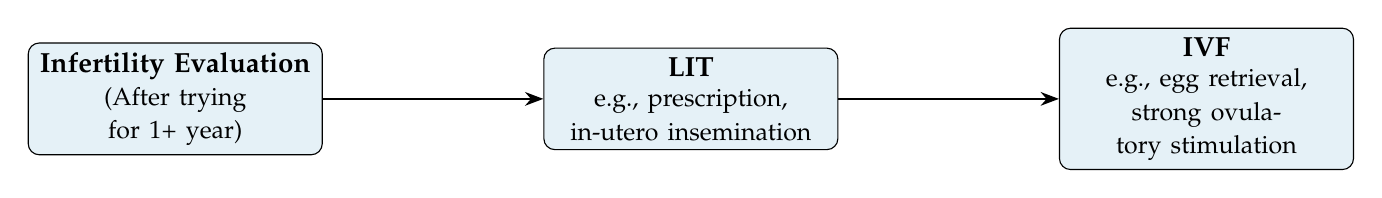
\begin{tikzpicture}[
    timeline/.style={
        draw, rounded corners, fill=blue!10, minimum height=1.2cm, text width=3.5cm, align=center
    },
    arrow/.style={-{Stealth}, thick},
    node distance=1.5cm and 2.8cm
]

% Nodes
\node[timeline] (eval) {\textbf{Infertility Evaluation}\\ \small (After trying for 1+ year)};
\node[timeline, right=of eval] (lit) {\textbf{LIT}\\ \small e.g., prescription,\\ in-utero insemination};
\node[timeline, right=of lit] (ivf) {\textbf{IVF}\\ \small e.g., egg retrieval,\\ strong ovulatory stimulation};

% Arrows
\draw[arrow] (eval) -- (lit);
\draw[arrow] (lit) -- (ivf);

\end{tikzpicture}%
}
\end{frame}

\begin{frame}{Data}
\begin{wideitemize}
\item \textbf{Swedish Population Register \& Statistics Sweden's longitudinal database}
	\begin{itemize}
		\item Individual level data with demographic and socioeconomic information, linked to their spouses (+ cohabiting partners).	
	\end{itemize}
\item \textbf{National Board of Health and Welfare}
	\begin{itemize}
		\item Link individual's all purchases of prescription drugs (name, classification code).
		\item University of inpatient hospital visits and specialist outpatient visits (date of visit, diagnosis codes).
		\item Universe of birth records (live, still, due date, gestational age at birth, resulted from a medically assisted conception).
	\end{itemize}
\end{wideitemize}	
\end{frame}

\begin{frame}{Sum stat: Final sample}
	\begin{figure}
		\resizebox{0.95\textheight}{!}{
			\includegraphics{tab1.png}
		}
	\end{figure}
\end{frame}

\begin{frame}
	\begin{center}
		\huge{The consequences of persistent infertility}
	\end{center}
\end{frame}

\begin{frame}{Empirical specification: Impact of persistent infertility}
	\vspace{1em}
	The paper first employs DiD-ish specification to estimate the impact of persistent infertility.
	\vspace{1em}
	\begin{block}{\textbf{Setup}}
		\begin{enumerate}
			\item \textbf{Sample}: Women who initiate any ART and conceive within 3 years of initiation.
			\item \textbf{Variation}: \textbf{(i)} women whose first conception after ART initiation resulted in a live birth and \textbf{(ii)} women whose first conception resulted in a miscarriage or stillbirth (``failed'').
			\item \textbf{Identification assumption}: Women whose first conception succeeds vs women whose first conception fails would have evolved over time in the counterfactual scenario.
		\end{enumerate}	
	\end{block}
	\begin{align*}
		\overbrace{Y_{it}}^{\hidewidth \text{Individual-level outcome} \hidewidth} = \alpha_i + \sum_{\tau} \kappa_{\tau} \underbrace{D_{\tau, it}}_{\hidewidth \text{FE: relative time} \hidewidth} + \sum_{\tau} \textcolor{red}{\sigma_{\tau}} D_{\tau,it} * Failed_i + \gamma_t + \beta * X_{it} + \varepsilon_{it}.
	\end{align*}

	\begin{itemize}
		\item $\gamma$: Time relative to the quarter (or year) of conception.
	\end{itemize}
\end{frame}

\begin{frame}{Results: Mental health}

	\begin{figure}
		\resizebox{0.8\textwidth}{!}{
		\includegraphics{men1.png}}
	\end{figure}

\end{frame}

\begin{frame}{Results: Income}

	\begin{figure}
		\resizebox{0.8\textwidth}{!}{
		\includegraphics{men2.png}}
	\end{figure}

\end{frame}

\begin{frame}{Results: Divorce rate}

	\begin{figure}
		\resizebox{0.8\textwidth}{!}{
		\includegraphics{men3.png}}
	\end{figure}

\end{frame}

\begin{frame}{Results: Summary}
\begin{wideitemize}
	\item Persistent infertility is bad for women's mental health.
	\item Persistent infertility has no ``protective'' long-run effect on women's income.
	\item \textcolor{red}{This is relative comparison between women who revealed their preference for having a child.} We are saying nothing about women who does not want to have a child having infertility.
	\item Persistent infertility leads to higher rates of divorce (\textcolor{red}{``child''-oriented family?}).
	\item ``Wanting to have a child'' might be the key here.

\end{wideitemize}	
\end{frame}

\begin{frame}
	\begin{center}
		\huge{Demand for infertility treatment}
	\end{center}
\end{frame}

\begin{frame}{Empirical specification: Impact of insurance coverage}
	The paper employ RDD to estimate the impact of insurance coverage on IVF initiation.\vspace{1em}

	\begin{block}{\textbf{Setup}}
		\begin{enumerate}
			\item \textbf{Sample}: Women-year-month panel around the age cut-off (2 yrs) for insurance coverage (as-if-random treatment).	
			\item \textbf{Running variable}: Regional age cut-off for insurance coverage.
			\item \textbf{Identifying assumption}: Age-based eligibility change is forseeable, but patients cannot perfectly control the timing of their treatment around the age cutoff (Really?).
		\end{enumerate}
	
	\end{block}

	\begin{align}
		\underbrace{Y_{itc}}_{\hidewidth \text{\hspace{3em} Initiating IVF treatment} \hidewidth} = \beta_0 + \textcolor{red}{\beta_1}\mathbb{1} [ a_{it} > \overbrace{A_{ct}}^{\hidewidth \text{Age cutoff} \hidewidth} ] + \beta_2 (a_{it} - A_{ct}) + \beta_3 \mathbb{1} [a_{it} > A_{ct}] \times (a_{it} - A_{ct}) + x'_{itc} \kappa + \varepsilon_{itc}\nonumber
	\end{align}
\end{frame}

\begin{frame}{Graphical evidence}
	\begin{columns}
		\begin{column}{0.5\textwidth}
		\resizebox{\textwidth}{!}{
			\includegraphics{rdd1.png}
		}
	\end{column}	
		\begin{column}{0.5\textwidth}
		\resizebox{\textwidth}{!}{
			\includegraphics{rdd2.png}
		}
	\end{column}	
\end{columns}\vspace{2em}

	\begin{wideitemize}
	\item Huge drop happening at the age cutoff.
	\end{wideitemize}
\end{frame}

\begin{frame}{Formal RDD estimates}
	\begin{figure}
		\resizebox{0.75\textwidth}{!}{
		\includegraphics{tab3.png}}
	\end{figure}
	
\end{frame}

\begin{frame}{Results: Summary}
\begin{wideitemize}
\item As women age out of insurance coverage, their rate of IVF initiation drops by 51\%. 

\end{wideitemize}	
\end{frame}

\end{document}
